\documentclass[]{article}
\usepackage{lmodern}
\usepackage{amssymb,amsmath}
\usepackage{ifxetex,ifluatex}
\usepackage{fixltx2e} % provides \textsubscript
\ifnum 0\ifxetex 1\fi\ifluatex 1\fi=0 % if pdftex
  \usepackage[T1]{fontenc}
  \usepackage[utf8]{inputenc}
\else % if luatex or xelatex
  \ifxetex
    \usepackage{mathspec}
    \usepackage{xltxtra,xunicode}
  \else
    \usepackage{fontspec}
  \fi
  \defaultfontfeatures{Mapping=tex-text,Scale=MatchLowercase}
  \newcommand{\euro}{€}
\fi
% use upquote if available, for straight quotes in verbatim environments
\IfFileExists{upquote.sty}{\usepackage{upquote}}{}
% use microtype if available
\IfFileExists{microtype.sty}{%
\usepackage{microtype}
\UseMicrotypeSet[protrusion]{basicmath} % disable protrusion for tt fonts
}{}
\usepackage[margin=1in]{geometry}
\usepackage{color}
\usepackage{fancyvrb}
\newcommand{\VerbBar}{|}
\newcommand{\VERB}{\Verb[commandchars=\\\{\}]}
\DefineVerbatimEnvironment{Highlighting}{Verbatim}{commandchars=\\\{\}}
% Add ',fontsize=\small' for more characters per line
\usepackage{framed}
\definecolor{shadecolor}{RGB}{248,248,248}
\newenvironment{Shaded}{\begin{snugshade}}{\end{snugshade}}
\newcommand{\KeywordTok}[1]{\textcolor[rgb]{0.13,0.29,0.53}{\textbf{{#1}}}}
\newcommand{\DataTypeTok}[1]{\textcolor[rgb]{0.13,0.29,0.53}{{#1}}}
\newcommand{\DecValTok}[1]{\textcolor[rgb]{0.00,0.00,0.81}{{#1}}}
\newcommand{\BaseNTok}[1]{\textcolor[rgb]{0.00,0.00,0.81}{{#1}}}
\newcommand{\FloatTok}[1]{\textcolor[rgb]{0.00,0.00,0.81}{{#1}}}
\newcommand{\CharTok}[1]{\textcolor[rgb]{0.31,0.60,0.02}{{#1}}}
\newcommand{\StringTok}[1]{\textcolor[rgb]{0.31,0.60,0.02}{{#1}}}
\newcommand{\CommentTok}[1]{\textcolor[rgb]{0.56,0.35,0.01}{\textit{{#1}}}}
\newcommand{\OtherTok}[1]{\textcolor[rgb]{0.56,0.35,0.01}{{#1}}}
\newcommand{\AlertTok}[1]{\textcolor[rgb]{0.94,0.16,0.16}{{#1}}}
\newcommand{\FunctionTok}[1]{\textcolor[rgb]{0.00,0.00,0.00}{{#1}}}
\newcommand{\RegionMarkerTok}[1]{{#1}}
\newcommand{\ErrorTok}[1]{\textbf{{#1}}}
\newcommand{\NormalTok}[1]{{#1}}
\ifxetex
  \usepackage[setpagesize=false, % page size defined by xetex
              unicode=false, % unicode breaks when used with xetex
              xetex]{hyperref}
\else
  \usepackage[unicode=true]{hyperref}
\fi
\hypersetup{breaklinks=true,
            bookmarks=true,
            pdfauthor={Prasanna K R},
            pdftitle={On Average, are Diamonds Certified by HRD Priced Higher than those Certified by Other Organizations?},
            colorlinks=true,
            citecolor=blue,
            urlcolor=blue,
            linkcolor=magenta,
            pdfborder={0 0 0}}
\urlstyle{same}  % don't use monospace font for urls
\setlength{\parindent}{0pt}
\setlength{\parskip}{6pt plus 2pt minus 1pt}
\setlength{\emergencystretch}{3em}  % prevent overfull lines
\setcounter{secnumdepth}{5}

%%% Use protect on footnotes to avoid problems with footnotes in titles
\let\rmarkdownfootnote\footnote%
\def\footnote{\protect\rmarkdownfootnote}

%%% Change title format to be more compact
\usepackage{titling}

% Create subtitle command for use in maketitle
\newcommand{\subtitle}[1]{
  \posttitle{
    \begin{center}\large#1\end{center}
    }
}

\setlength{\droptitle}{-2em}
  \title{On Average, are Diamonds Certified by HRD Priced Higher than those
Certified by Other Organizations?}
  \pretitle{\vspace{\droptitle}\centering\huge}
  \posttitle{\par}
  \author{Prasanna K R}
  \preauthor{\centering\large\emph}
  \postauthor{\par}
  \predate{\centering\large\emph}
  \postdate{\par}
  \date{August 31, 2015}



\begin{document}

\maketitle


\section{The Hypotheses}\label{the-hypotheses}

Let us state our Hypotheses:

\begin{itemize}
\itemsep1pt\parskip0pt\parsep0pt
\item
  Null Hypothesis (H\textsubscript{0}) : On average, there is no
  difference in diamond's pricing, between HRD or any other organization
\item
  Alternate Hypothesis (H\textsubscript{A}): On average, HRD certified
  diamonds are priced higher (one-sided test)
\end{itemize}

Mathematically, the hypothese are expressed below:

\begin{itemize}
\itemsep1pt\parskip0pt\parsep0pt
\item
  H\textsubscript{0}: μ\textsubscript{diff} = 0
\item
  H\textsubscript{A}: μ\textsubscript{diff} \textgreater{} 0
\end{itemize}

\section{The Data}\label{the-data}

We separate the data sets - diamonds certified by HRD and other
diamonds. There are \texttt{79} observations of HRD Diamonds and
\texttt{229} non-HRD Certified Diamonds.

\section{Central Limit Theorm: Checking the Conditions for Hypothesis
Testing for Paired
Data}\label{central-limit-theorm-checking-the-conditions-for-hypothesis-testing-for-paired-data}

The conditions for hypothesis testing:

\begin{itemize}
\itemsep1pt\parskip0pt\parsep0pt
\item
  Independence: Sampled observations must be independent. Random sample
  must be collected with replacement because the size of HRD Certified
  diamond is small
\item
  Sample Size / Skew: The no of elements must be more than 30.
\end{itemize}

We select a size of 40 with replacement.

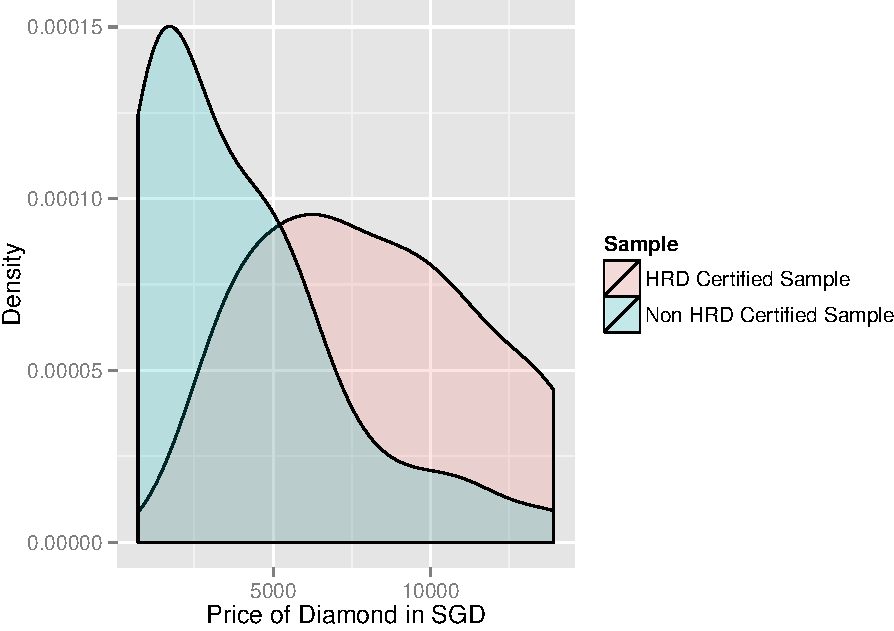
\includegraphics[width=450px]{DiamondHypothesis_files/figure-latex/vizualize-1}
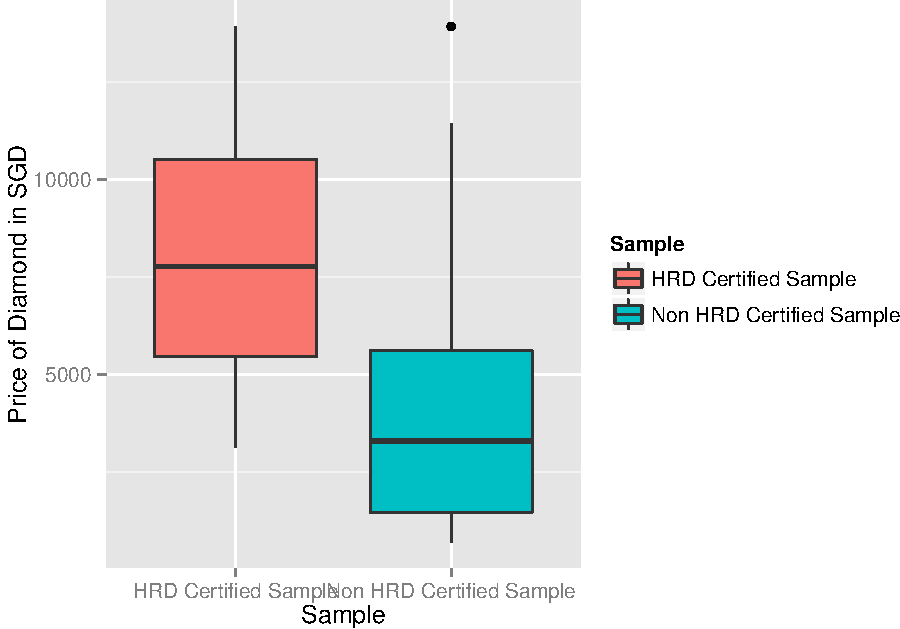
\includegraphics[width=450px]{DiamondHypothesis_files/figure-latex/vizualize-2}

\section{The Test Statistic}\label{the-test-statistic}

\begin{Shaded}
\begin{Highlighting}[]
\NormalTok{zScore <-}\StringTok{ }\NormalTok{xBar /}\StringTok{ }\KeywordTok{standardError}\NormalTok{(Diff)}
\NormalTok{zScore}
\end{Highlighting}
\end{Shaded}

\begin{verbatim}
## [1] 5.758039
\end{verbatim}

\begin{Shaded}
\begin{Highlighting}[]
\CommentTok{# Calculating p-value}
\CommentTok{# 1-pnorm() because we are doing a one-sided test - greater than}
\NormalTok{pValue <-}\StringTok{ }\DecValTok{1}\NormalTok{-}\KeywordTok{pnorm}\NormalTok{( zScore ) }
\NormalTok{pValue}
\end{Highlighting}
\end{Shaded}

\begin{verbatim}
## [1] 0.000000004254841
\end{verbatim}

\section{Null Hypothesis (H\textsubscript{0}) is
Rejected}\label{null-hypothesis-h0-is-rejected}

The \textbf{Null Hypothesis (H\textsubscript{0})} is rejected because
the pValue is lesser than the significance value of 0.05.

\end{document}
